\documentclass[11pt]{article}


\usepackage{fullpage}
\usepackage{graphicx}
\usepackage{amsmath}
\usepackage{amssymb}
\usepackage{amsthm}
\usepackage{fancyvrb}

\newcommand{\myname}{Mehshan Mustafa}

\newenvironment{theorem}[2][Theorem]{\begin{trivlist}
\item[\hskip \labelsep {\bfseries #1}\hskip \labelsep {\bfseries #2.}]}{\end{trivlist}}
\newenvironment{lemma}[2][Lemma]{\begin{trivlist}
\item[\hskip \labelsep {\bfseries #1}\hskip \labelsep {\bfseries #2.}]}{\end{trivlist}}
\newenvironment{exercise}[2][Exercise]{\begin{trivlist}
\item[\hskip \labelsep {\bfseries #1}\hskip \labelsep {\bfseries #2.}]}{\end{trivlist}}
\newenvironment{problem}[2][Problem]{\begin{trivlist}
\item[\hskip \labelsep {\bfseries #1}\hskip \labelsep {\bfseries #2.}]}{\end{trivlist}}
\newenvironment{question}[2][Question]{\begin{trivlist}
\item[\hskip \labelsep {\bfseries #1}\hskip \labelsep {\bfseries #2.}]}{\end{trivlist}}
\newenvironment{corollary}[2][Corollary]{\begin{trivlist}
\item[\hskip \labelsep {\bfseries #1}\hskip \labelsep {\bfseries #2.}]}{\end{trivlist}}
\newenvironment{solution}{\begin{proof}[Solution]}{\end{proof}}
\newenvironment{idea}[2][Proof Idea.]{\textit{#1} #2}



\parindent0in
\pagestyle{plain}
\thispagestyle{plain}

\newcommand{\dated}{\today}

\begin{document}

\textbf{Introduction to the Theory of
Computation}\hfill\textbf{\myname}\\[0.01in]
\textbf{Chapter 2: Context-Free Languages}\hfill\textbf{\dated}\\
\smallskip\hrule\bigskip

\begin{problem}{2.24}
Let $E = \{a^{i}b^{j} \ | \ i \neq j \ and \ 2i \neq j \}$. Show that $E$ is a context-free language.
\end{problem}

\begin{idea}
There are four cases when we take into account the parity of $i$ and $j$: 
\begin{enumerate}
\item If $j$ is odd, then accept if $i \neq j$.
\item If $i$ is odd and $j$ is even, then accept if $2i \neq j$.
\item If both $i$ and $j$ are even, then accept if $i > j$.
\item If both $i$ and $j$ are even, then accept if $i < j$.
\end{enumerate}
\end{idea}

\begin{proof}
Proof is by construction. Construct a PDA that non-deterministically tests the four cases mentioned above to recognize the language $E$.
\end{proof}

\begin{center}
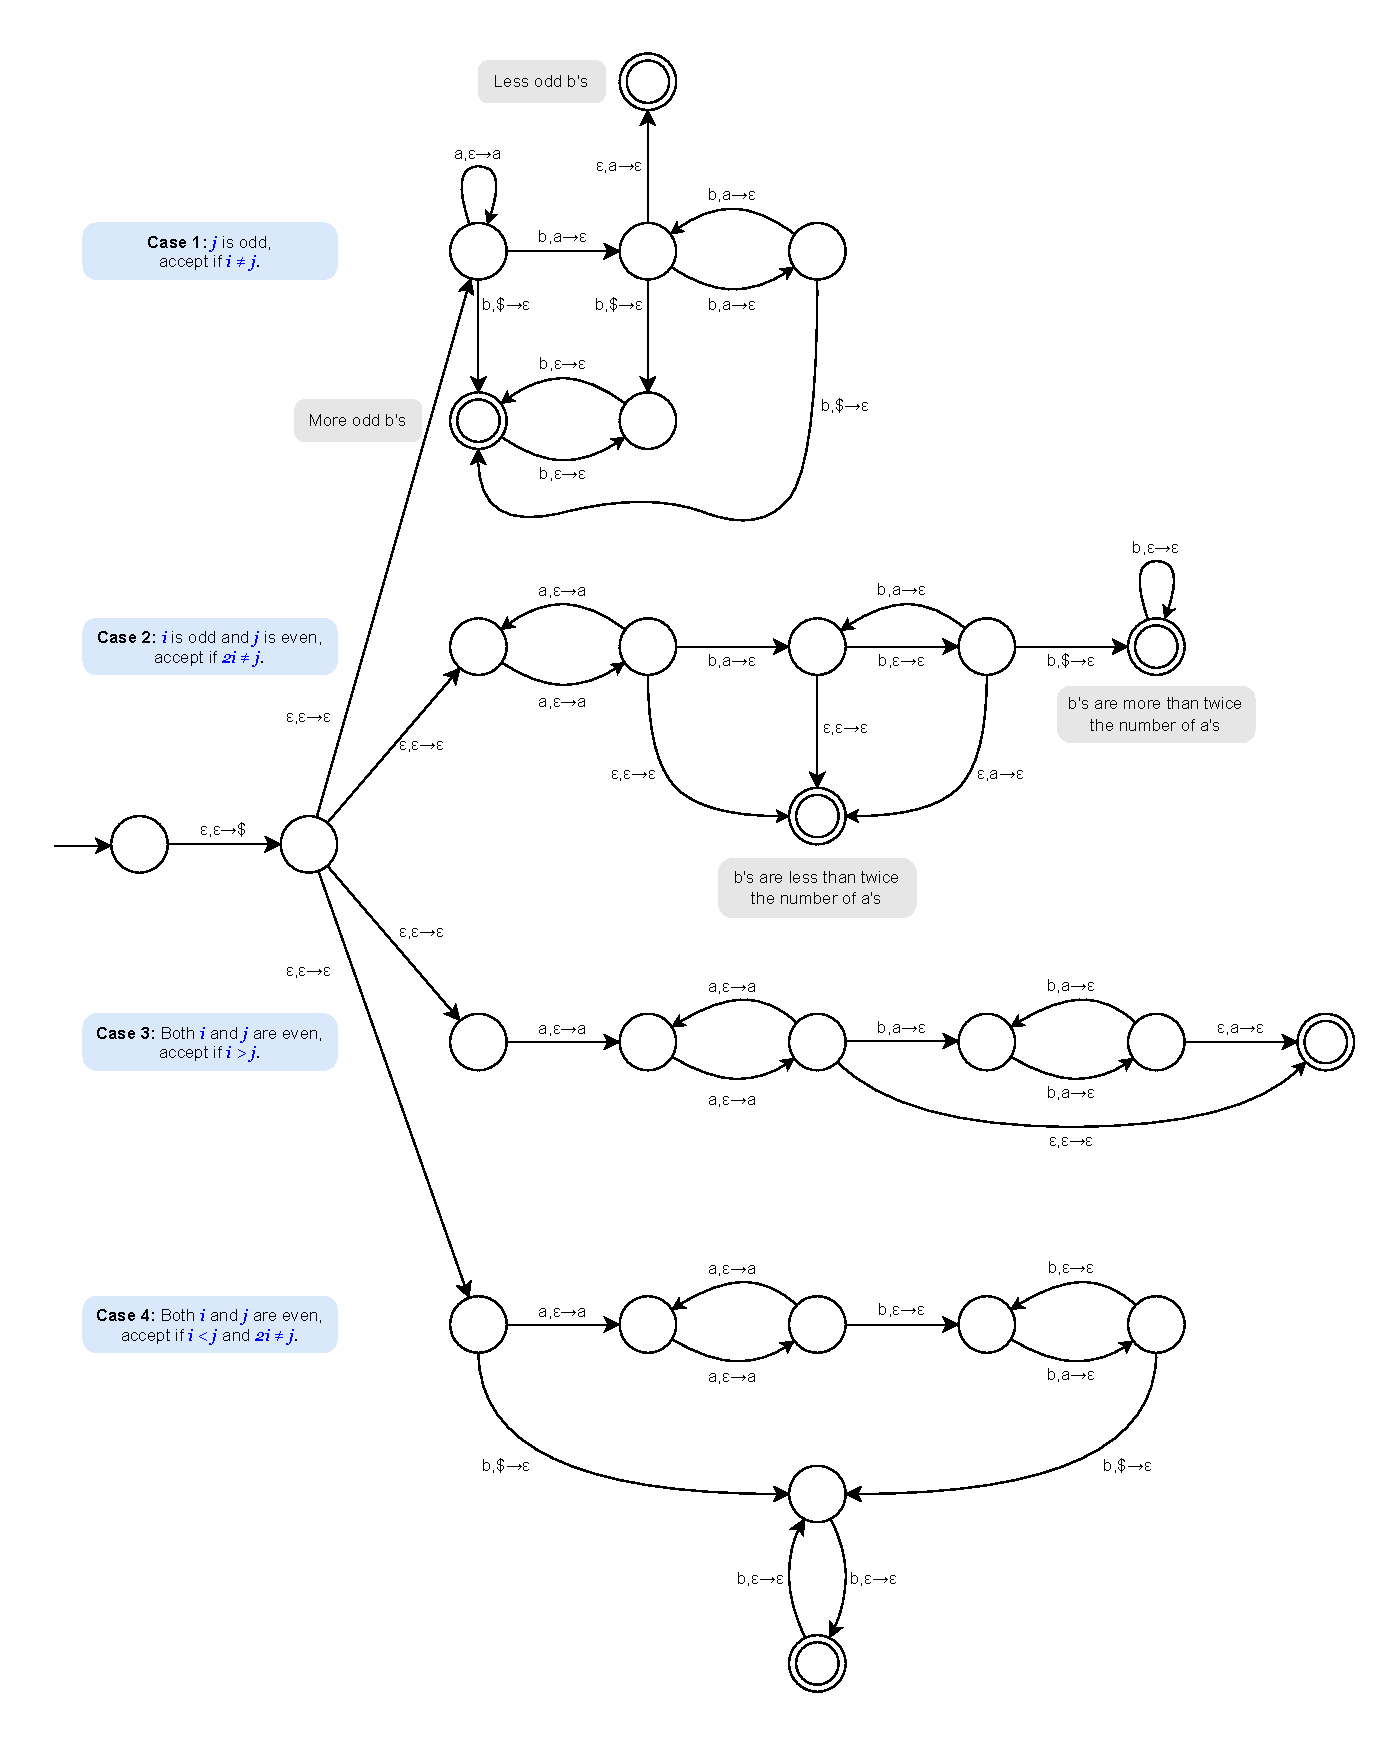
\includegraphics[scale=0.7]{Figures/Problem2.24.pdf} \\
A PDA that recognizes $E$. It non-deterministically tests the four cases based on the parity of $i$ and $j$.
\end{center}

\end{document}
